\chapter{モジュール情報及び品質試験結果管理システム}
前章で述べたように、モジュール生産及び品質試験を世界中で行う。
これらの情報はデータベースシステムを用いて管理することが決定していて、現在この開発を行っている。
システムについては、ITkの全情報を保存する中央データベースと、各組み立て期間に設置し、データ管理を行うローカルデータベースである。
本章ではこれらのデータベースについて説明する。また、システム開発の中で私が開発を行った機能について詳細に説明する。

\section{中央データベース}
\subsection{中央データベースの概要}
\subsubsection{概要}
中央データベースは、ITkの製造に関する全ての情報の保存を目的として開発されたデータベースである。
ユニコーン大学が開発、運用を行っていて、チェコにデータベースサーバーが設けられている。
ITkは、ピクセル検出機とストリップ検出機にから構成される。
これらを生産するにあたって、シリコンセンサーや電気基板といった小さな部品から製造を行い、それらを用いたモジュールの組み立て、複数モジュールを搭載したstaveやringの組み立てを経て検出器が完成する。
また各組み立て段階において、動作確認等を目的とした品質試験を行う。
これらの過程における全ての構成部品の情報、及び品質試験結果を中央データベースに保存する。

\subsubsection{意義}
中央データベースに保存された情報は、検出器運転時の参考値として扱われる。
モジュールを例にだすと、品質試験で読み出し試験を行った際の最適な設定値を中央データベースに保存するため、実際の運転時に参照することができる。
また運転前の状態における検出器の性能、運転前後での検出機性能比較を行うことができる。

\subsection{モジュール情報構造および構成部品との関係の実装}
中央データベースにモジュールを登録するためには、モジュールの種類、その構成部品といった情報構造を決定し、データベース上に定義しておく必要がある。この情報構造をデータベースに実装し、登録できる仕組みを整えた。
詳細な種類と構造については表\ref{pd_module_structure}に示す。
またQuadモジュールに関する例を図\ref{example_module_structure}に示す。

\begin{table}[tbp]
\begin{center}
\caption[中央データベースにおけるモジュールの種類と構造一覧]{中央データベースにおけるモジュールの種類と構造一覧。中央データベースにモジュールを登録するときの情報として、モジュールの種類、構成部品を表のように実装した。Triplet、Quadというように、モジュールの種類ごとに登録できるシステムとなっており、PCBなどの対応する構成部品の紐付けも同時に行うことができる。}
\label{pd_module_structure}
  \begin{tabular}{|ll|} \hline
    種類 & 構成する部品(数) \\ \hline
    Triplet L0 stave module   &  Single bare module(3) \\
                              &  Triplet stave PCB(1) \\\hline
    Triplet L0 Ring0 module   &  Single bare module(3) \\
                              &  Triplet R0 PCB(1) \\\hline
    Triplet L0 Ring0.5 module &  Single bare module(3) \\
                              &  Triplet R0.5 PCB(1) \\\hline
    L1 quad module            &  Quad bare module(1) \\
                              &  Quad PCB(1) \\\hline
    Outer system quad moudle  &  Quad bare module(1) \\
                              &  Quad PCB(1) \\\hline
    Outer system quad moudle  &  Dual bare module(1) \\
                              &  Dual PCB(1) \\\hline
    Digital triplet L0 stave module   &  Digital single bare module(3) \\
                                      &  Triplet stave PCB(1) \\\hline
    Digital triplet L0 Ring0 module   &  Digital single bare module(3) \\
                                      &  Triplet R0 PCB(1) \\\hline
    Digital triplet L0 Ring0.5 module &  Digital single bare module(3) \\
                                      &  Triplet R0.5 PCB(1) \\\hline
    Digital quad module       &  Digital quad bare module(1) \\
                              &  Quad PCB(1) \\\hline
    Digital L1 quad moudle    &  Digital quad bare module(1) \\
                              &  Quad PCB(1) \\\hline
    Dummy triplet L0 stave module   &  Dummy single bare module(3) \\
                                    &  Triplet stave PCB(1) \\\hline
    Dummy triplet L0 Ring0 module   &  Dummy single bare module(3) \\
                                    &  Triplet R0 PCB(1) \\\hline
    Dummy triplet L0 Ring0.5 module &  Dummy single bare module(3) \\
                                    &  Triplet R0.5 PCB(1) \\\hline
    Dummy quad module       &  Dummy quad bare module(1) \\
                            &  Quad PCB(1) \\\hline
    Dummy L1 quad moudle    &  Dummyl quad bare module(1) \\
                            &  Quad PCB(1) \\ \hline
  \end{tabular}
\end{center}
\end{table}

\begin{figure}[bpt]\centering
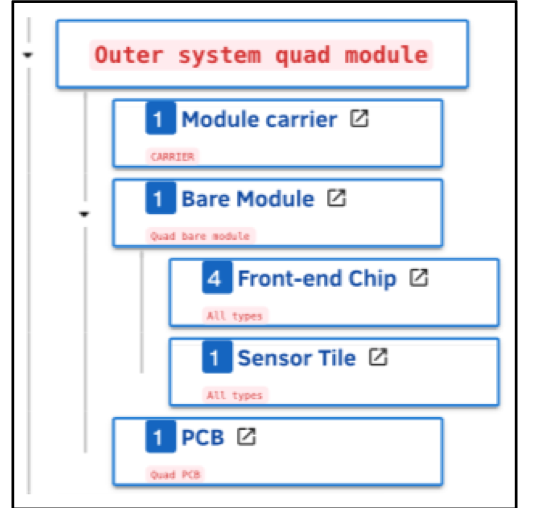
\includegraphics[width=7cm]{example_module_structure}
\caption[中央データベース内におけるモジュール構造の一例(Quadモジュール)]{中央データベース内におけるモジュール構造の一例(Quadモジュール)。例としてOuter system quad moduleの中央データベース内の構造を示している。この種類では構成要素としてそれぞれ対応する種類のModule carrier、Bare Module、PCBを持つことがわかる。さらにBare ModuleはFE chipを4、Sensorを1持つことが分かり、Quadモジュールの構造が正しく実装されていることが分かる。}
\label{example_module_structure}
\end{figure}

\subsection{組み立て工程および品質試験の情報形式の実装}
モジュールの情報構造の実装に加えて、品質試験の情報を正確に管理するには、モジュール組み立て工程と付随する品質試験の項目をデータベース上に定義する必要がある。
これを実装し、試験結果を適切な組み立て工程へアップロードできる仕組みを整えた。

詳細な構造を図\ref{pd_stage_structure}に示す。

\begin{table}[tbp]
\begin{center}
\caption[中央データベースにおける組み立て工程と付随するテスト項目]{中央データベースにおける組み立て工程と付随するテスト項目。モジュールの組み立て工程及び品質試験を登録するため、表のような構造を実装した。データベース内でこの表に沿った組み立て工程の登録、更新、試験結果のアップロードができるようになった。}
\label{pd_stage_structure}
  \begin{tabular}{|ll|} \hline
    組み立て項目 & 付随する組み立て情報及び品質試験項目 \\ \hline
    1. Bare to PCB assembly & Visual Inspection \\ 
                            & Metrology \\
                            & Mass measurement \\
                            & Glue information \\\hline
    2. Wirebonding          & Visual Inspection \\ 
                            & Wirebond information \\
                            & (Wirebond pull test)\\
                            & First power up\\
                            & Sensor IV\\
                            & SLDO VI\\
                            & Chip configuration\\
                            & Pixel failure test\\\hline

    3. Wirebond Protection  & Visual Inspection \\ 
                            & Potting information \\
                            & Sensor IV \\
                            & Register test\\
                            & Readout for basic electrical \\\hline

    4. Parylene Coating     & Visual Inspection \\ 
                            & Palylene information \\
                            & Mass measurement \\
                            & Sensor IV \\
                            & Register test\\
                            & Readout for basic electrical \\
                            & Bump bond quality \\\hline

    5. Thermal Cycling      & Visual Inspection \\ 
                            & Thermal cycling info \\
                            & Sensor IV \\
                            & Register test\\
                            & Readout for basic electrical \\
                            & Bump bond quality \\\hline

    6. Burn-in              & Visual Inspection \\ 
                            & Metrology \\
                            & Mass Measurement \\
                            & First power up\\
                            & Sensor IV\\
                            & SLDO VI\\
                            & Chip configuration\\
                            & Pixel failure test\\\hline

    7. Reception            & \\\hline 
  \end{tabular}
\end{center}
\end{table}

\newpage

\section{ローカルデータベース}
\subsection{ローカルデータベースの概要と意義}
中央データベースでは、前述したようにモジュールの情報のみならずITkに関わるすべての情報を管理する。データベースの機能としては汎用的に使えるようなものになっている。
モジュールの組み立て及びその品質試験に関しては3章で述べたように工程が複数に渡り、行う品質試験の数も多い。
1つの生産現場で多いところでは数千個のモジュールを作ることになるため、
データ管理が簡単にかつ円滑に進むようになっているのが好ましい。
このような理由から、生産現場での生産性、利便性に特化し、円滑な生産をサポートすることを目的としたデータベースシステム(ローカルデータベース)を開発している。
システムの概要図を図\ref{localdb_overview}に示す。オープンソースのサービスであるMongoDB\cite{4-1}と、開発を行っっているローカルデータベース用ウェブアプリケーションを併用することでデータ管理や中央データベースとの同期を行うシステムとなっている。

\begin{figure}[bpt]\centering
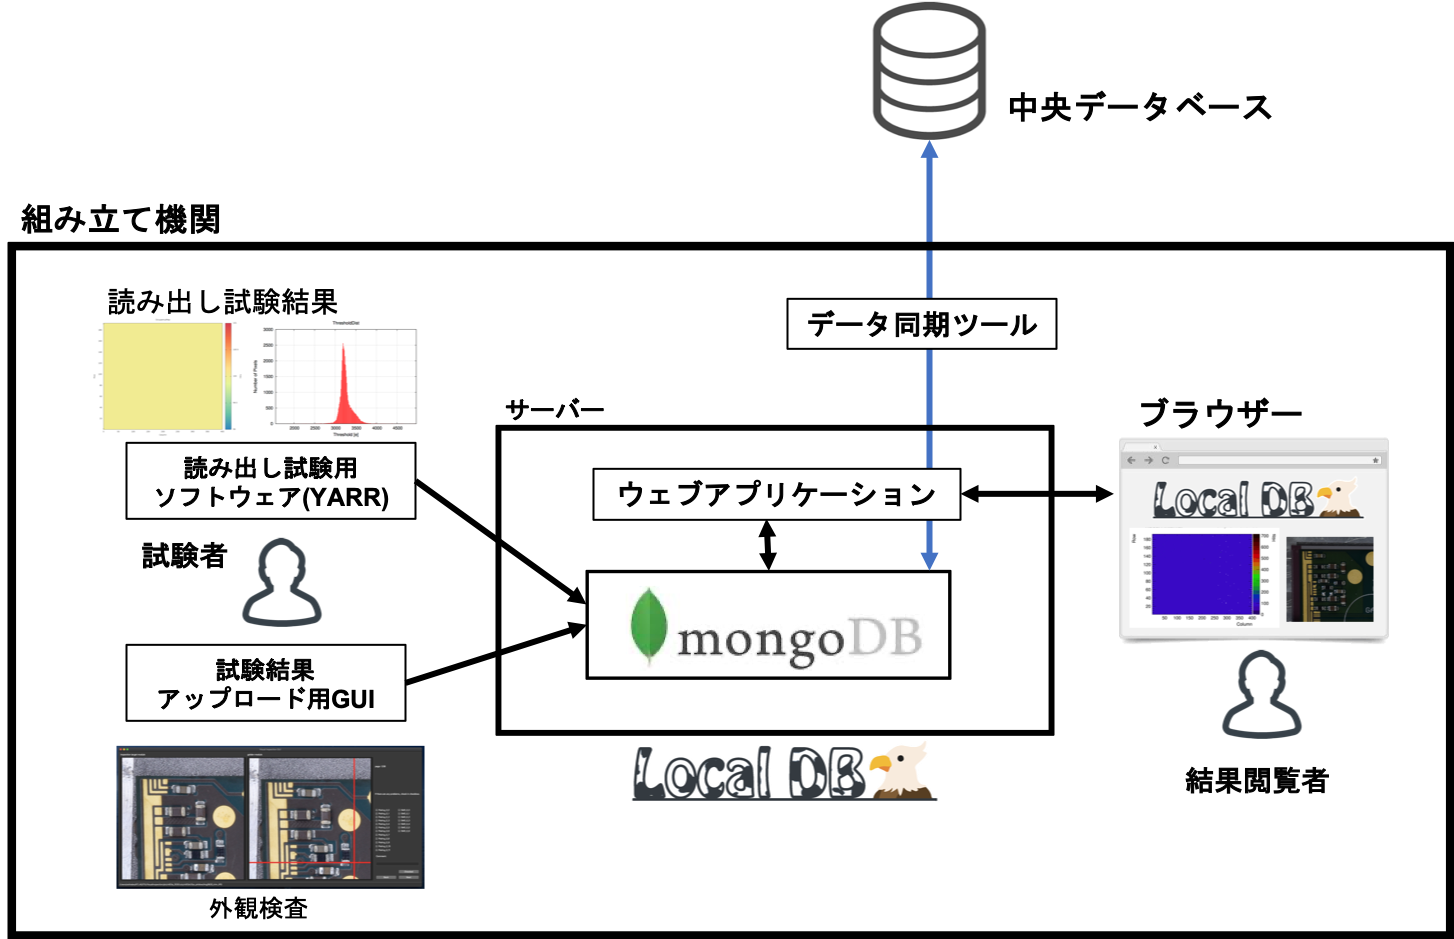
\includegraphics[width=15cm]{localdb_overview}
\caption[ローカルデータベースシステムの概要]{ローカルデータベースシステムの概要。各組み立て機関でMongoDBとローカルデータベース用ウェブアプリケーションの立ち上げを行い、独自にデータ管理をするシステムとなっている。品質試験者は図のようにいくつかのソフトウェアを用いて試験結果をMongoDBに保存する。保存された結果はウェブアプリケーションによって閲覧することができる。また結果は中央データベースに集める必要があるため、同期ツールを用いて試験結果の共有を行う。}
\label{localdb_overview}
\end{figure}

具体的にローカルデータベースは以下のような利点を持つ。

\begin{itemize}
  \item ローカルにデータベースサーバーを立てるためアクセス速度が早く、円滑にデータ管理を行うことができる。
  \item モジュールの組み立て工程を管理し、生産者の適切な処理を助ける。
  \item モジュールに特化したデータ管理、解析を行うことで異常をいち早く検知できる。
  \item 試験者の情報や試験時間など、品質試験結果以外の必要な情報を正確に管理できる。
\end{itemize}

\subsection{MongoDBと内部構造\cite{4-2}}
MongoDBとはNoSQLに分類されるデータベースである。
MongoDBの構造について簡単に表したものを図\ref{mongodb_schema}に示す。
一般的なSQLDBのようにテーブル形式ではなく、JSON形式で情報を格納する。
情報を保持している一枚のシートをドキュメントと呼び、コレクションと呼ばれる枠に複数のドキュメントが格納されている。
各ドキュメントはIDを持っていて、異なるコレクションにおけるドキュメント間の紐付けはこのIDを用いて行う。

\begin{figure}[bpt]\centering
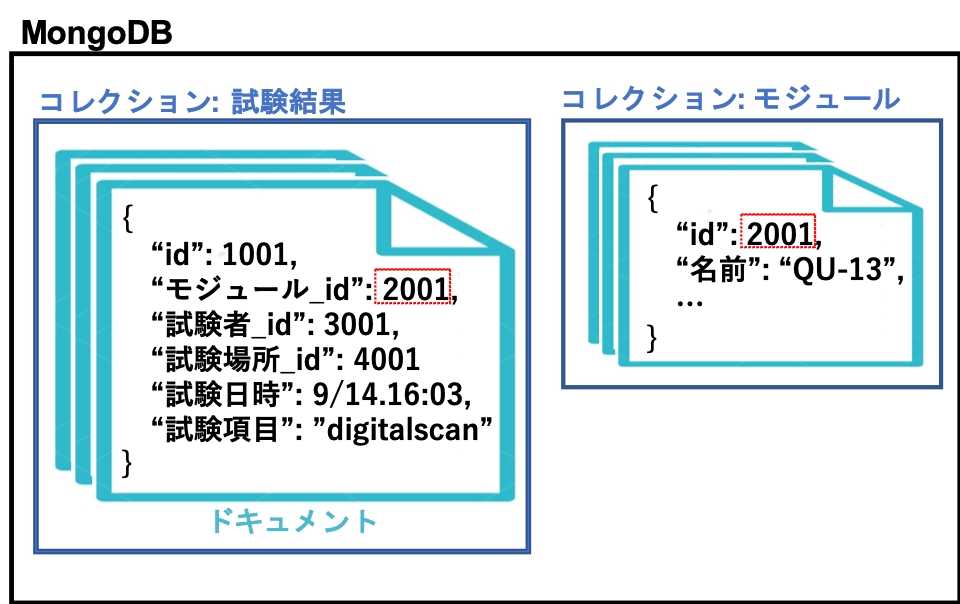
\includegraphics[width=10cm]{mongodb_schema}
\caption[MongoDBの構造の例\cite{4-2}]{MongoDBの構造の例\cite{4-2}。図のようにMongoDBではJSON形式でデータを格納する。1枚のシートをドキュメントと呼び、複数のドキュメントが格納されている枠組みをコレクションと呼ぶ。ドキュメントの構造及びコレクション間の関係等を決めることでデータベースの構造を定義する。}
\label{mongodb_schema}
\end{figure}

ローカルデータベースシステムにおいて、MongoDBを使用する主な利点を以下に示す。

\begin{itemize}
  \item 各コレクションに格納するドキュメントの構造が動的であるため、開発を柔軟に行うことができる。
  \item JSON形式でデータを保持するため情報取得の際の整形処理が不要で、ウェブアプリケーションとの親和性が高い。
  \item 全ての処理をメモリ上で実行するため、高速な読み書きが可能。
\end{itemize}

モジュール及び品質試験に用いる主なコレクションと内部情報を表\ref{localdb_structure}に示す。

\begin{table}[tbp]
\begin{center}
\caption[品質試験に用いる主なコレクション]{品質試験に用いる主なコレクション。ローカルデータベースシステムにおいて、MongoDB内に2つのデータベースを設置し、使用する。}
\label{localdb_structure}
  \begin{tabular}{|lll|} \hline
    データベース名 & コレクション名 & 情報 \\ \hline
    localdb      & component & モジュール情報、FEチップ情報 \\ 
                 & childParentRelation & FEチップとモジュールの関係性 \\ 
                 & QC.module.status & 各モジュールに対する組み立て工程及び選択された試験結果 \\ 
                 & QC.result & 品質試験結果 \\ 
                 & testRun & 読み出し試験結果 \\ 
                 & user & 読み出し試験実施者 \\
                 & institute & 読み出し試験実施場所 \\
                 & componentTestRun & componentとtestRunの関係性 \\
                 & comments & コメント情報 \\ \hline
    localdbtools & QC.status & 組み立て工程及び試験項目\\
                 & viewer.user & 登録ユーザの情報 \\
                 & viewer.query & 読み出し結果キーワード、検索機能実行時に使用 \\ 
                 & viewer.tag.docs & モジュールや試験結果に付けるタグの情報 \\ \hline
  \end{tabular}
\end{center}
\end{table}

\subsection{データ同期ツール}
モジュールや品質試験の結果のデータ共有のために、中央データベースとローカルデータベースの間でデータ同期が行われる必要がある。
これを行うツールをPythonを用いて開発した。現在は以下のような機能を実装している。
\begin{itemize}
  \item モジュール情報のダウンロード
  \item 読み出し試験結果のアップロード
\end{itemize}
実装した開発項目について、詳細については以下で述べる。
読み出し試験以外に実施する品質試験結果のダウンロード、アップロードの機能や、組み立て工程情報の取得等の機能が今後の開発課題として上げられる。

\subsection{ウェブアプリケーション}
各組み立て機関において、試験者が品質試験結果を閲覧、管理するツールとして、ウェブアプリケーションを開発している。
ローカルデータベースとアプリケーション間の処理に特化したイメージを図\ref{webapp_process}に示す。
このようにアプリケーションはデータベースとブラウザー、データベース間のインターフェースとなっている。

\begin{figure}[bpt]\centering
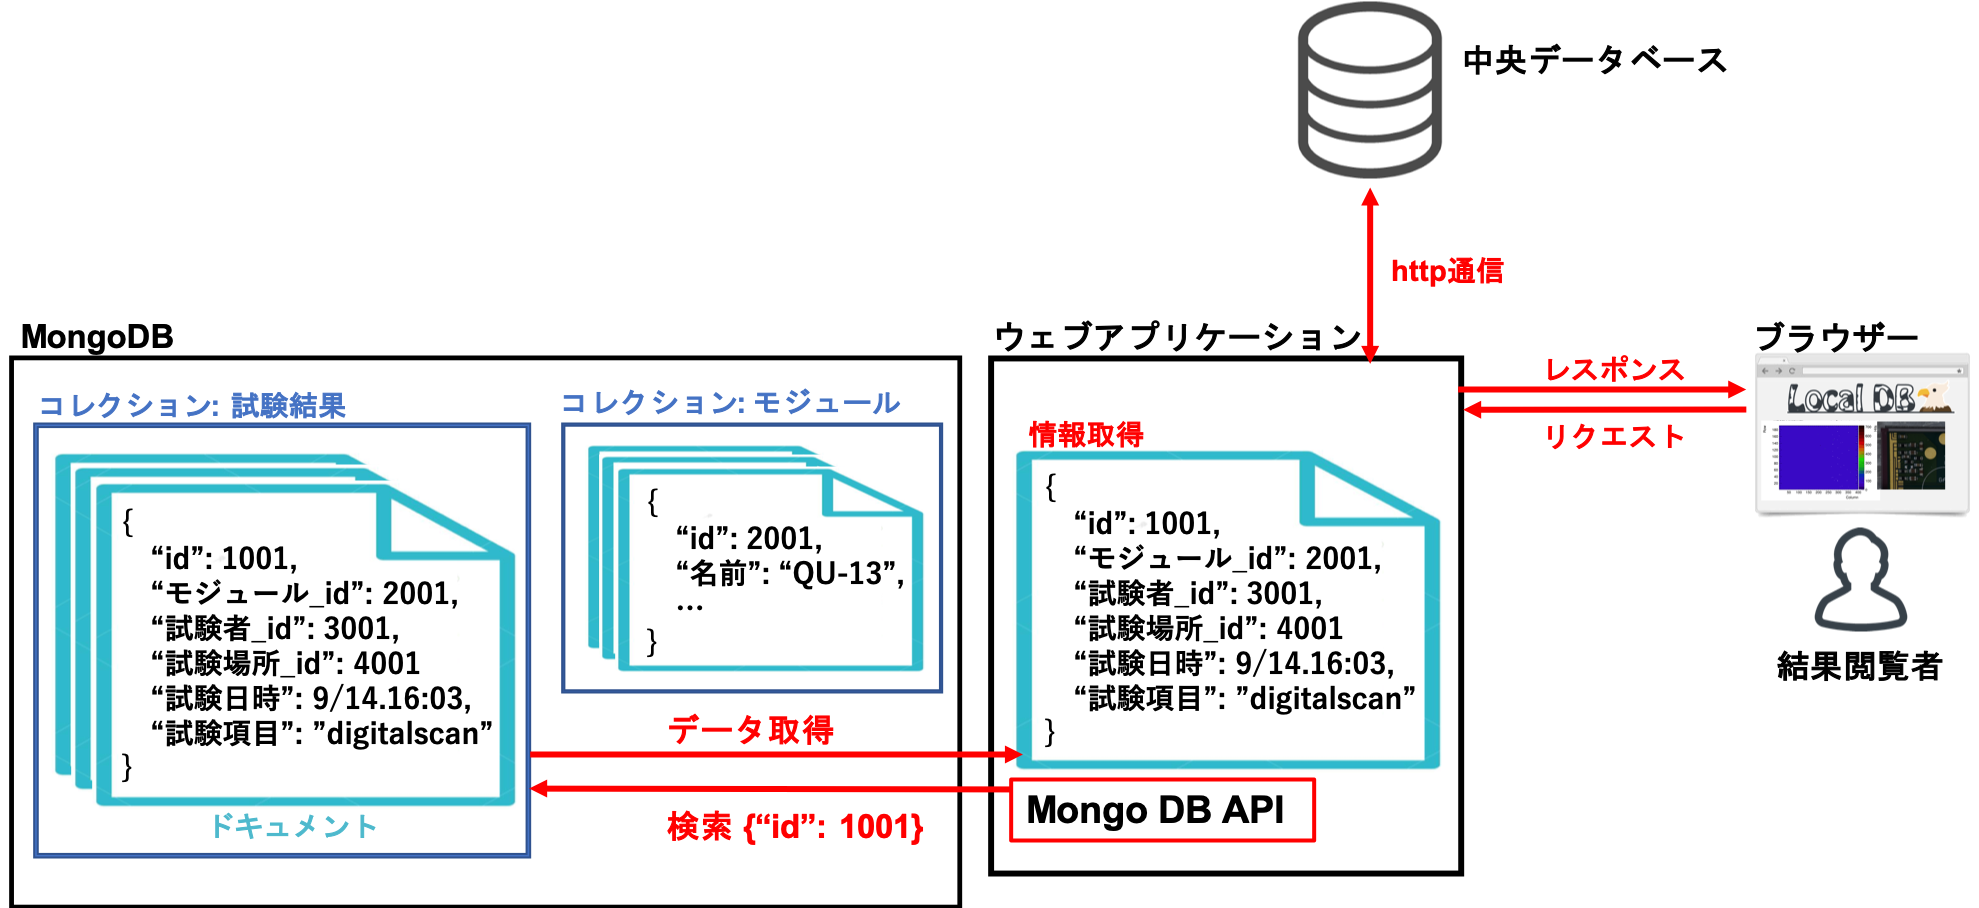
\includegraphics[width=16cm]{webapp_process}
\caption[ウェブアプリケーション処理のイメージ]{ウェブアプリケーション処理のイメージ。ウェブアプリケーションではMongoDBのAPIを用いて、データベースのコレクションに検索をかけることで情報を取得する。取得した情報は整形されたのちブラウザに送信、中央データベースとの同期等の処理に用いられる。}
\label{viewer_result}
\end{figure}

試験結果を迅速に分かりやすく見るシステムを作り、円滑な生産の補助や異常結果の早期発見を目的としている。
またデータベースの情報管理のみならず、同期ツールや、後述する試験結果解析ツールなどの外部スクリプトの実行、結果取得等、生産時における多くのデータベース操作はこのアプリケーションを用いて行う。

ウェブアプリケーションでは、現在以下の機能を使用することができる。ある品質試験の結果ページを図\ref{viewer_result}に示す。

\begin{itemize}
  \item 登録モジュール情報及び品質試験結果の閲覧、解析
  \item ローカルデータベースにおけるユーザ管理機能
  \item 上述した同期処理実行機能
\end{itemize}

\begin{figure}[bpt]\centering
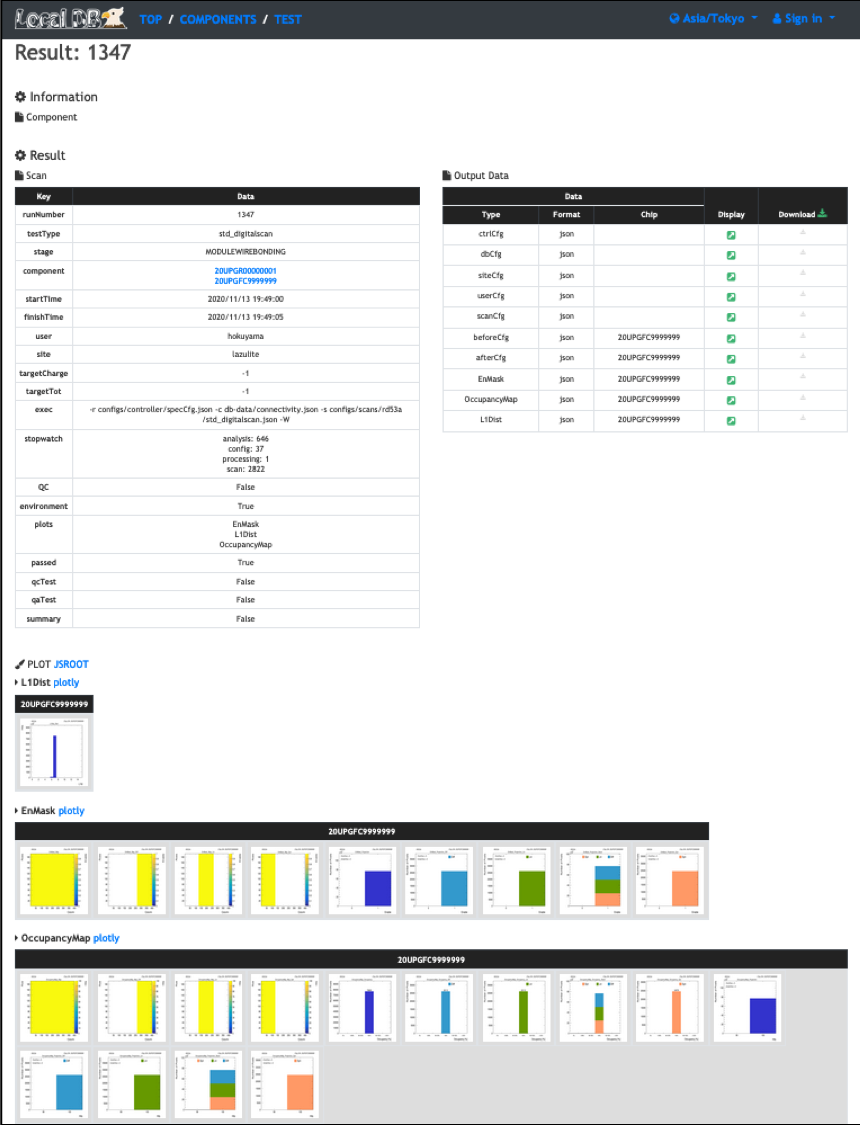
\includegraphics[width=10cm]{viewer_result}
\caption[品質試験結果ページの例]{品質試験結果ページの例。図は品質試験項目であるデジタル回路読み出しの結果を表している。図の上部に試験情報や設定値、下部に結果のグラフが表示されているのを確認できる。}
\label{viewer_result}
\end{figure}

\newpage
\section{チュートリアルと普及状況}
ローカルデータベースの機能の普及を目的として、2020年2月にCERN研究所にてシステムのチュートリアルを行った。
このチュートリアルは以下のような2つのセッションに分けて行った。

\begin{itemize}
  \item 参加者が実際にサーバーの設定、各ソフトウェアのインストールを行いながら機能を実践するセッション(2月3日から6日まで)
  \item 私が参加者の前で実際に機能を実践し、システムや使い方に対して議論を行うセッション(2月7日)
\end{itemize}

それぞれのセッションの様子を図\ref{Tutorial_picture}に示す。
数多くの議論を行い、有益なフィードバックを得ることができた。
また品質試験の流れにおいて、一連の機能確認をすることができた。

\begin{figure}[bpt]
  \begin{center}
  \begin{minipage}{0.4\hsize}
    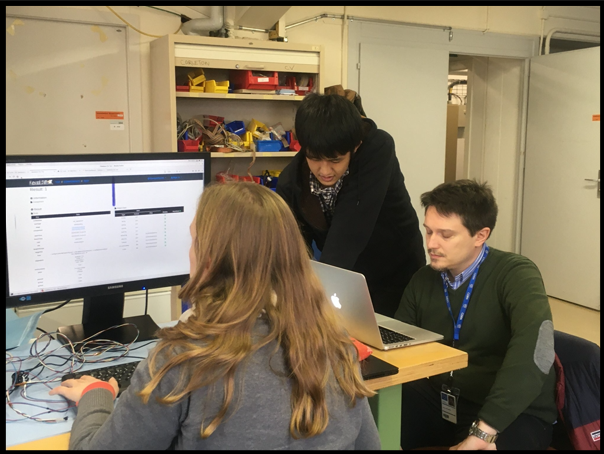
\includegraphics[width=6cm]{hands_on}
  \end{minipage}
  \begin{minipage}{0.4\hsize}
    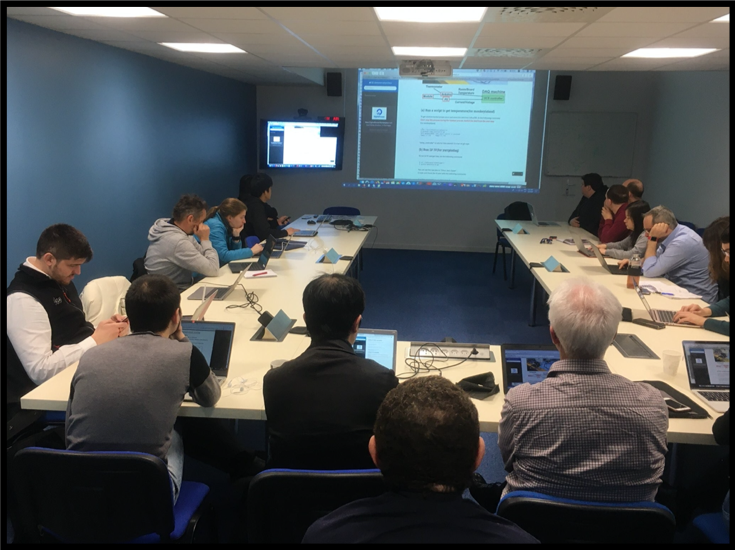
\includegraphics[width=6cm]{hands_off}
  \end{minipage}
  \caption[ローカルデータベースシステムチュートリアルの様子]{ローカルデータベースシステムチュートリアルの様子。2020年2月にCERNでローカルデータベースシステムのチュートリアルを行った。参加者が実際にシステムの設置、機能実行を行うハンズオンセッション(左図)と、参加者の前で実際に機能の動作をみせ、議論を行うハンズオフセッション(右図)に分けて行った。システムに有益な情報を獲得したと共に、システムの機能普及に成功した。}
  \label{Tutorial_picture}
  \end{center}
\end{figure}

これを経て現在ローカルデータベースは世界18箇所にて導入され、試験運用が開始している。
将来的には全組み立て機関で使うことが決定しており、それに向けたシステム開発、サポートが必要となっている状況である。
ローカルデータベースについて、導入及び試験運用を行っている機関を以下に示す。また世界地図を\ref{localdb_world_map}に示す。

\begin{itemize}
  \item 高エネルギー加速器研究機構(KEK), 日本
  \item 欧州原子核研究機構(CERN), スイス
  \item University of Liverpool, イギリス
  \item University of Oxford, イギリス
  \item University of Glasgow, イギリス
  \item Paris-Saclay University, フランス
  \item パリ第6大学, フランス
  \item フランス国立科学研究センター, フランス
  \item University of Grenoble, フランス
  \item University of Gottingen, ドイツ
  \item University of Siegen, ドイツ
  \item University of Genoa, イタリア
  \item University of Salento, イタリア
  \item University of Milan, イタリア
  \item University of Udine, イタリア
  \item Univerity of Trento, イタリア
  \item University of Oklahoma, アメリカ
  \item Argonne National Laboratory, アメリカ
  \item Lawrence Berkeley National Laboratory(LBL), アメリカ
\end{itemize}

\begin{figure}[bpt]\centering
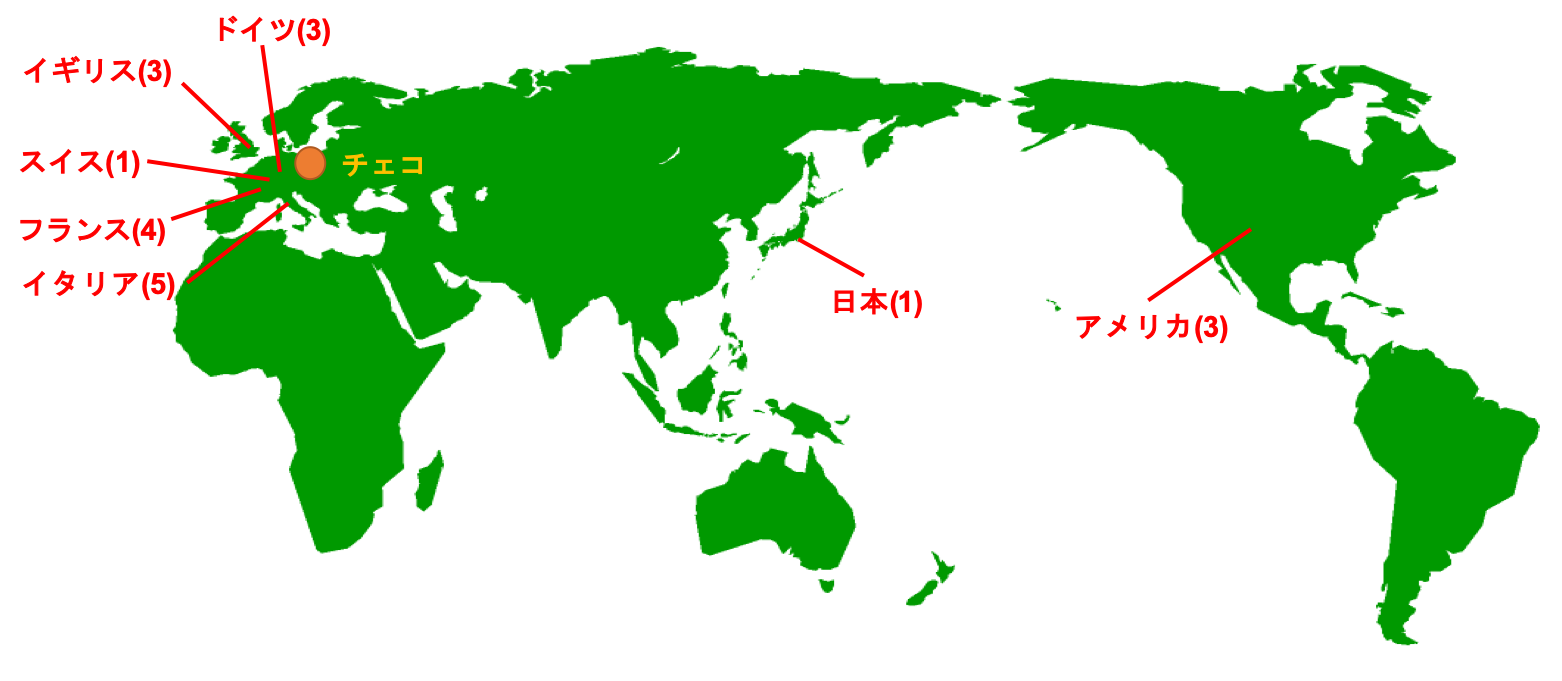
\includegraphics[width=14cm]{localdb_world_map}
\caption[ローカルデータベースシステム導入及び試運転場所]{ローカルデータベースシステム導入及び試運転場所。赤文字は設置している地域、括弧内の数字はその地域におけるシステム導入場所の数を示している。2020年11月現在、ローカルデータベースシステムは世界18の機関で試験運転がなされている。日本を除いてその多くはヨーロッパとアメリカに位置していることが分かる。}
\label{localdb_world_map}
\end{figure}

%%%%%%%%%%%%%%%%%%%%%%%%%%%%%%%%%%%%%%%%%%%%%%%%%%%%%%%
%%%%%%%%%%%%%%%%%%%%%%%%%%%%%%%%%%%%%%%%%%%%%%%%%%%%%%%
%%%%%%%%%%%%%%%%%%%%%%%%%%%%%%%%%%%%%%%%%%%%%%%%%%%%%%%
\clearpage
\section{実装した機能}
私は、このシステムの中に以下のような機能を実装した。詳細について以下に述べる。
\begin{itemize}
  \item ユーザ管理機能
  \item 品質試験結果の登録と組み立て工程の管理機能
  \item 読み出し試験におけるピクセル解析ツール
  \item 読み出し試験結果検索機能
  \item 中央データベースとの同期ツール
\end{itemize}

%%%%%%%%%%%%%%%%%%%%%%%%%%%%%%%%%%%%%%%%%%%%%%%%%%%%%%%
%%%%%%%%%%%%%%%%%%%%%%%%%%%%%%%%%%%%%%%%%%%%%%%%%%%%%%%
\subsection{ユーザ管理機能及び各種機能}

異常があった際に確認することを目的として、誰が試験を行ったかを記録することが必要である。
また、モジュールの登録や中央データベースとの同期など、データベースの機能使用を制限することも必要である。
これらを目的として、試験者及びデータベース使用者情報の管理システムを開発、実装した。
この詳細について以下に述べる。

\subsubsection{機能概要}
データベース権限の段階として、管理者、権限付きユーザ、一般ユーザの3段階を設けた。
各ユーザが使うことのできる機能を表\ref{user_functions_summary}に示す。

\begin{table}[tbp]
\begin{center}
\caption[ローカルデータベースユーザ権限及び使用機能一覧]{ローカルデータベースユーザ権限及び使用機能一覧。ローカルデータシステムにおけるユーザとして、管理者、権限付きユーザ、一般ユーザの3つを設けた。全てのユーザがウェブアプリケーションの閲覧をすることができる。管理者、権限付きユーザにはデータベース読み書き権限とウェブアプリケーションログイン権限が与えられ、試験結果のアップロード、アプリケーション上のユーザ機能の実行ができる。また管理者は権限付きユーザを登録することができる。}
\label{user_functions_summary}
  \begin{tabular}{|lll|} \hline
    ユーザ       & 付加される権限                               & 使用できる機能 \\ \hline
    管理者       & ユーザ管理権限                     & 権限付きユーザ登録機能\\ 
                 & データベース読み書き権限           & \\ 
                 & ウェブアプリケーションログイン権限 & \\ \hline
    権限付ユーザ & データベース読み書き権限           & 試験結果のアップロード\\ 
                 & ウェブアプリケーションログイン権限 & 中央データベースとのデータ同期機能\\ 
                 &                                    & その他ウェブアプリケーションの機能(コメント、タグ)\\ \hline
    一般ユーザ   &                                    & モジュール情報及び試験結果の閲覧 \\ \hline
  \end{tabular}
\end{center}
\end{table}

権限付きユーザの機能としてモジュール及び試験結果にコメント、タグをつける機能を実装した。使用したときの様子を図\ref{webapp_comment}、\ref{webapp_tag}に示す。

\begin{figure}[bpt]\centering
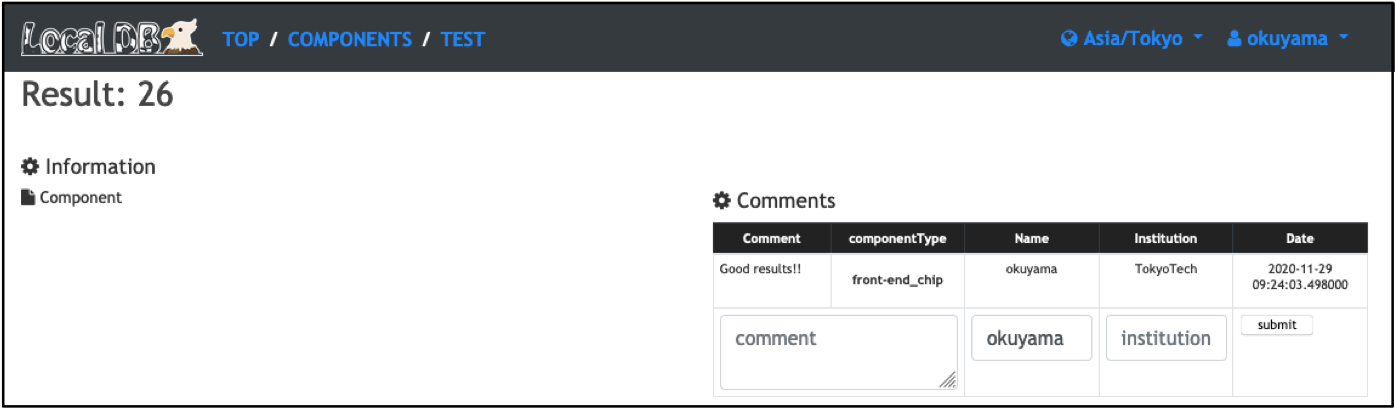
\includegraphics[width=12cm]{viewer_comment}
\caption[ウェブアプリケーションにおけるコメント機能]{ウェブアプリケーションにおけるコメント機能。権限付きユーザ及び管理者はモジュールや試験結果に対してコメントをすることができる。図のようにページの右側にコメント欄があり、コメントをテキスト形式で記述することができる。}
\label{webapp_comment}
\end{figure}

\begin{figure}[bpt]\centering
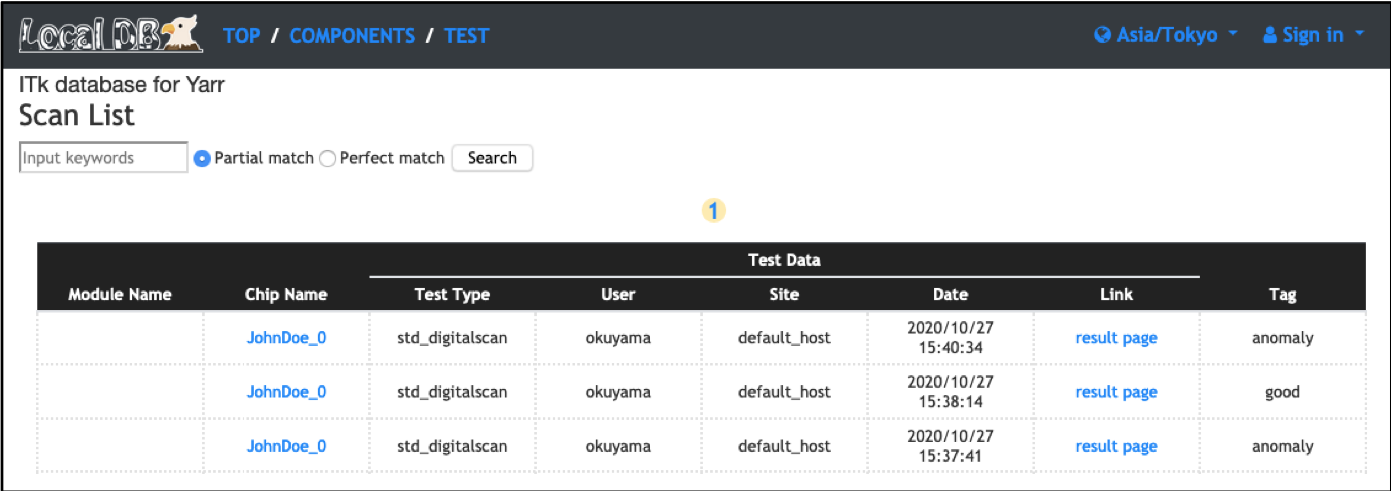
\includegraphics[width=12cm]{viewer_tag}
\caption[ウェブアプリケーションにおけるタグ機能]{ウェブアプリケーションにおけるタグ機能。権限付きユーザ及び管理者はモジュールや試験結果に対してタグをつけることができる。図は試験結果の一覧ページであり、図の表において一番右の列がつけられたタグを示しており、図ではanomalyやgoodといったタグが付けられていることが分かる。}
\label{webapp_tag}
\end{figure}

\subsubsection{ユーザ登録操作}
表\ref{user_functions_summary}において管理者と権限付ユーザの登録について説明する。

データベースシステム導入時に管理者のアカウントを作成する。
コマンドプロンプト上で開発したスクリプトを用いて実行することで管理者登録がなされ、この際ユーザ名とパスワードを入力する。

権限付ユーザについて、全ての品質試験者及びデータベースユーザ機能使用者は管理者によってユーザ登録される必要がある。
登録はウェブアプリケーションを用いて行い、以下の情報を入力する。
\begin{itemize}
  \item ユーザ名 
  \item 氏名
  \item 所属機関
  \item メールアドレス 
\end{itemize}

管理者が登録を完了すると、登録されたメールアドレスに登録完了メールと仮パスワードが届く。
このメールに従い、ウェブアプリケーション上でユーザがパスワード登録を完了する。

このようにメール機能を用いることでパスワード漏洩の防止、管理者操作の削減を目的としている。

\subsubsection{機能の仕組み}
ユーザ登録の際には内部で以下の2つの処理が行われるように実装した。

\begin{enumerate}
  \item MongoDBアカウントの作成、読み書き権限の付与
  \item ウェブアプリケーションで用いるユーザ情報ドキュメントの作成
\end{enumerate}

1の処理を行う理由は、登録ユーザが試験結果をmongoDBにアップロードできるようにするためである。
2の情報は、ウェブアプリケーション内でのログイン判断、ユーザの情報保持に使う。
この情報は表\ref{localdb_structure}のviewer.userに保存される。
2つの処理について、実際に保存されるドキュメントの例をリスト\ref{user_doc_1}、\ref{user_doc_2}以下に示す。

\begin{lstlisting}[caption=MongoDBアカウント情報を持つドキュメントの例。リスト中の"roles"より、localdbとlocaldbtoolsの読み書き権限が付加されていることが分かる。,label=user_doc_1]
{
	"_id" : "localdb.hokuyama",
	"userId" : UUID("fee321eb-83b8-434a-a4a0-fff638b5db36"),
	"user" : "hokuyama",
	"db" : "localdb",
	"credentials" : {
		"SCRAM-SHA-1" : {
			"iterationCount" : 10000,
			"salt" : "smkhqvrYnxtsN7rvdadw8g==",
			"storedKey" : "6wC3HyeGTN4px+FV839ou1bylp0=",
			"serverKey" : "/sUu8aX86hnvvMvNq9tC+WZHTDE="
		},
		"SCRAM-SHA-256" : {
			"iterationCount" : 15000,
			"salt" : "RCC51GuZ4IQK+fINo5HDKP4Vp6LPdersp2gmIA==",
			"storedKey" : "+WwblqTl/SvyyiP7H867kMPPh3Uy2wRIeQ2PgCpdWzs=",
			"serverKey" : "651T+2BkP1FE4YEHKbxf+JTnzsR9yWcZQPA/y9RN8e0="
		}
	},
	"roles" : [
		{
			"role" : "readWrite",
			"db" : "localdb"
		},
		{
			"role" : "readWrite",
			"db" : "localdbtools"
		}
	]
}
\end{lstlisting}
\begin{lstlisting}[caption=ウェブアプリケーションで扱うユーザ情報を持つドキュメントの例。リスト\ref{user_doc_1}で示したものとは別に、ウェブアプリケーション内でユーザ情報を扱うためにこのドキュメントを保持する必要がある。ウェブにおいてログインはこのドキュメントの存在確認をもってなされる。パスワードはhash化して保存している。,label=user_doc_2]
{
	"_id" : ObjectId("5f0bbe84ef87af2628865de7"),
	"sys" : {
		"rev" : 0,
		"cts" : ISODate("2020-07-13T10:53:07.943Z"),
		"mts" : ISODate("2020-07-13T10:53:07.943Z")
	},
	"username" : "hokuyama",
	"name" : "Hiroki Okuyama",
	"auth" : "readWrite",
	"institution" : "Tokyo Institute of Technology",
	"Email" : "okuyama@hep.phys.titech.ac.jp",
	"password" : "5f4dcc3b5aa765d61d8327deb882cf99"
}
\end{lstlisting}

%%%%%%%%%%%%%%%%%%%%%%%%%%%%%%%%%%%%%%%%%%%%%%%%%%%%%%%
%%%%%%%%%%%%%%%%%%%%%%%%%%%%%%%%%%%%%%%%%%%%%%%%%%%%%%%
\newpage
\subsection{品質試験結果の登録と組み立て工程の自動更新}
ローカルデータベースへアップロードした品質試験結果の中から、本結果として中央データベースへアップロードする結果を選択する機能を開発した。
品質試験は各モジュール、各組み立て工程に対して行うものであるため、結果選択も同様に工程毎に行うことを想定している。
結果選択後、データベースにおける組み立て工程の情報は次のものへ自動的に更新する機能となっている。

\subsubsection{概要}
あるモジュール、組み立て工程に対して結果を選択する様子を図\ref{webapp_sign_off}に示す。組み立て工程も自動更新されていることがわかる。

\begin{figure}[bpt]\centering
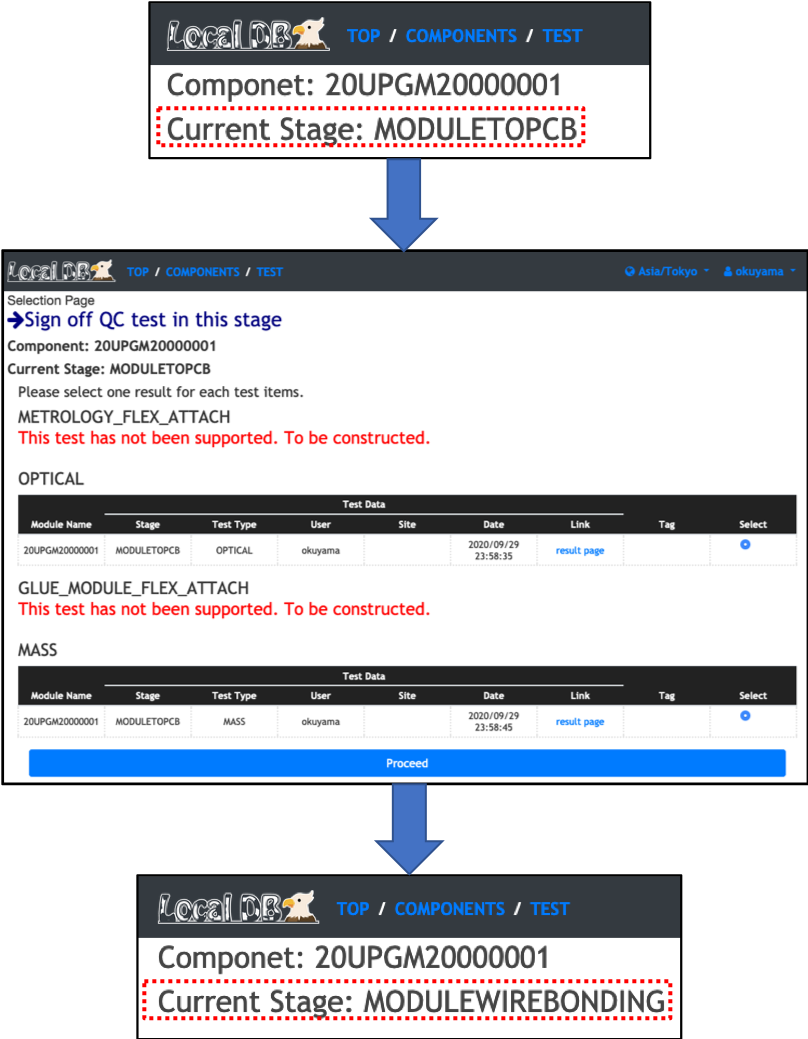
\includegraphics[width=10cm]{webapp_sign_off}
\caption[結果選択画面及び組み立て工程表示の例]{結果選択画面及び組み立て工程表示の例。図の上部で組み立て工程が"MODULETOPCB"である。この段階において結果を選択する処理を行うとローカルデータベース内で選択された結果にタグ付けがなされる。図の中部においてその処理を行なっており、この図では"OPTICAL"と"MASS"の結果を選択している。選択した結果は中央データベースと同期される。また結果選択後は組み立て工程が自動的に更新される。図の下部では"MODULEWIREBONDING"になっていることが分かる。}
\label{webapp_sign_off}
\end{figure}

\newpage
\subsubsection{仕組み}
リスト\ref{qc_status}、\ref{qc_module_status}のようなドキュメントを作成、保存する。
リスト\ref{qc_status}は全てのモジュールに対して共通のドキュメントであり、組み立て工程と各工程における品質試験項目を記録する。
これらの情報は中央データベースより取得される。
この情報を参照することでローカルデータベース内部での組み立て工程の管理が可能となっている。

リスト\ref{qc_module_status}は各モジュールに対して1つ存在し、以下のような情報を保持する。
\begin{itemize}
  \item 現在工程
  \item 各工程における品質試験結果のID
\end{itemize}


\begin{lstlisting}[caption=組み立て工程及び品質試験一覧情報ドキュメント。このようなドキュメントを作成、保持しておくことで組み立て工程及び品質試験の情報を扱う。ローカルデータベース内に1つこのドキュメントを保持し、品質試験結果選択、組み立て工程の更新時にこのドキュメントを参照する。このドキュメントは中央データベースよりデータ取得して作成する。,label=qc_status]
{
	"_id" : ObjectId("5fc89aa232d56b29091fd64d"),
	"sys" : {
		"mts" : ISODate("2020-12-03T07:58:26.310Z"),
		"cts" : ISODate("2020-12-03T07:58:26.310Z"),
		"rev" : 0
	},
	"dbVersion" : 1.01,
	"proddbVersion" : 1.01,
	"stage_flow" : [
		"MODULETOPCB",
		"MODULEWIREBONDING",
		"MODULEWIREBONDPROTECTION",
		"MODULEPARYLENECOATING",
		"MODULETHERMALCYCLING",
		"MODULEBURNIN",
		"MODULERECEPTION"
	],
	"stage_test" : {
		"MODULETOPCB" : [
			"OPTICAL",
			"GLUE_MODULE_FLEX_ATTACH",
			"MASS",
			"METROLOGY"
		],
		"MODULEWIREBONDING" : [
			"WIREBONDING",
			"OPTICAL",
			"SENSOR_IV",
			"PIXEL_FAILURE_TEST",
			"SLDO_VI",
			"WIREBOND",
			"CHIP_CONFIGURATION"
		],
		"MODULEWIREBONDPROTECTION" : [
			"OPTICAL",
			"POTTING",
			"MASS",
			"READOUT_IN_BASIC_ELECTRICAL_TEST",
			"SENSOR_IV",
			"REGISTER_TEST"
		],
    ...
	},
...
}
\end{lstlisting}

\begin{lstlisting}[caption=モジュールの組み立て工程及び品質試験結果管理のためのドキュメント例。各モジュールにおいて現在の組み立て工程及び選択された品質試験結果がこのドキュメントに保存される。ドキュメント内の"currentStage"に現工程を保持する。また選択した試験結果のIDを"QC$\_$results"に各組み立て工程ごとに持つようになっている。,label=qc_module_status]
{
	"_id" : ObjectId("5fc4be4c12a45922a91b0e75"),
	"sys" : {
		"mts" : ISODate("2020-11-30T09:41:32.411Z"),
		"cts" : ISODate("2020-11-30T09:41:32.411Z"),
		"rev" : 0
	},
	"dbVersion" : 1.01,
	"proddbVersion" : 1.01,
	"component" : "5fa79114e615fa000a1a5976",
	"currentStage" : "MODULEWIREBONDPROTECTION",
	"latestSyncedStage" : "MODULEWIREBONDING",
	"status" : "created",
	"rework_stage" : [ ],
	"QC_results" : {
		"MODULETOPCB" : {
			"OPTICAL" : "5fc4c2cfb6c93d451e2c9ac1",
			"GLUE_MODULE_FLEX_ATTACH" : "-1",
			"MASS" : "5fc4c2da27766dc6e89c024f",
			"METROLOGY" : "5fc4c2eaf1f19d9cb5859f00"
		},
		"MODULEWIREBONDING" : {
			"WIREBONDING" : "-1",
			"OPTICAL" : "5fc4c4c8b7d0c86912b4958f",
			"SENSOR_IV" : "5fc4c59e9e283a57ccaa1088",
			"PIXEL_FAILURE_TEST" : "5fca342f6e9f1f5eafedfb92",
			"SLDO_VI" : "-1",
			"WIREBOND" : "-1",
			"CHIP_CONFIGURATION" : "-1"
		},
		"MODULEWIREBONDPROTECTION" : {
			"OPTICAL" : "-1",
			"POTTING" : "-1",
			"MASS" : "-1",
			"READOUT_IN_BASIC_ELECTRICAL_TEST" : "-1",
			"SENSOR_IV" : "-1",
			"REGISTER_TEST" : "-1"
		},
    ...
	}
}
\end{lstlisting}

%%%%%%%%%%%%%%%%%%%%%%%%%%%%%%%%%%%%%%%%%%%%%%%%%%%%%%%
%%%%%%%%%%%%%%%%%%%%%%%%%%%%%%%%%%%%%%%%%%%%%%%%%%%%%%%

\newpage
\subsection{読み出し試験結果におけるピクセル解析ツール}
節\ref{sec:pixel_analysis}で述べたように、読み出し試験ではピクセル解析を行う。
ローカルデータベースにアップロードされた結果を用いて、この解析を行うツールを開発した。
開発の詳細とツール確認のためのデモンストレーションについて5章で述べる。


%%%%%%%%%%%%%%%%%%%%%%%%%%%%%%%%%%%%%%%%%%%%%%%%%%%%%%%
%%%%%%%%%%%%%%%%%%%%%%%%%%%%%%%%%%%%%%%%%%%%%%%%%%%%%%%
\subsection{読み出し試験結果の検索機能}
登録モジュールや品質試験結果の一覧ページに検索機能を実装した。
確認したいモジュール情報や試験結果を迅速に取得し、閲覧できることを目的としている。検索機能を使用している様子を図\ref{webapp_search_function}に示す。

キーワードを入力し、検索することができる仕組みとなっていて、一般的なウェブページの検索エンジンのように扱うことができる。
現在は単一キーワード検索の他に、以下の機能を実装している。
\begin{itemize}
  \item 完全一致、部分一致検索
  \item AND、OR検索
\end{itemize}

\begin{figure}[bpt]\centering
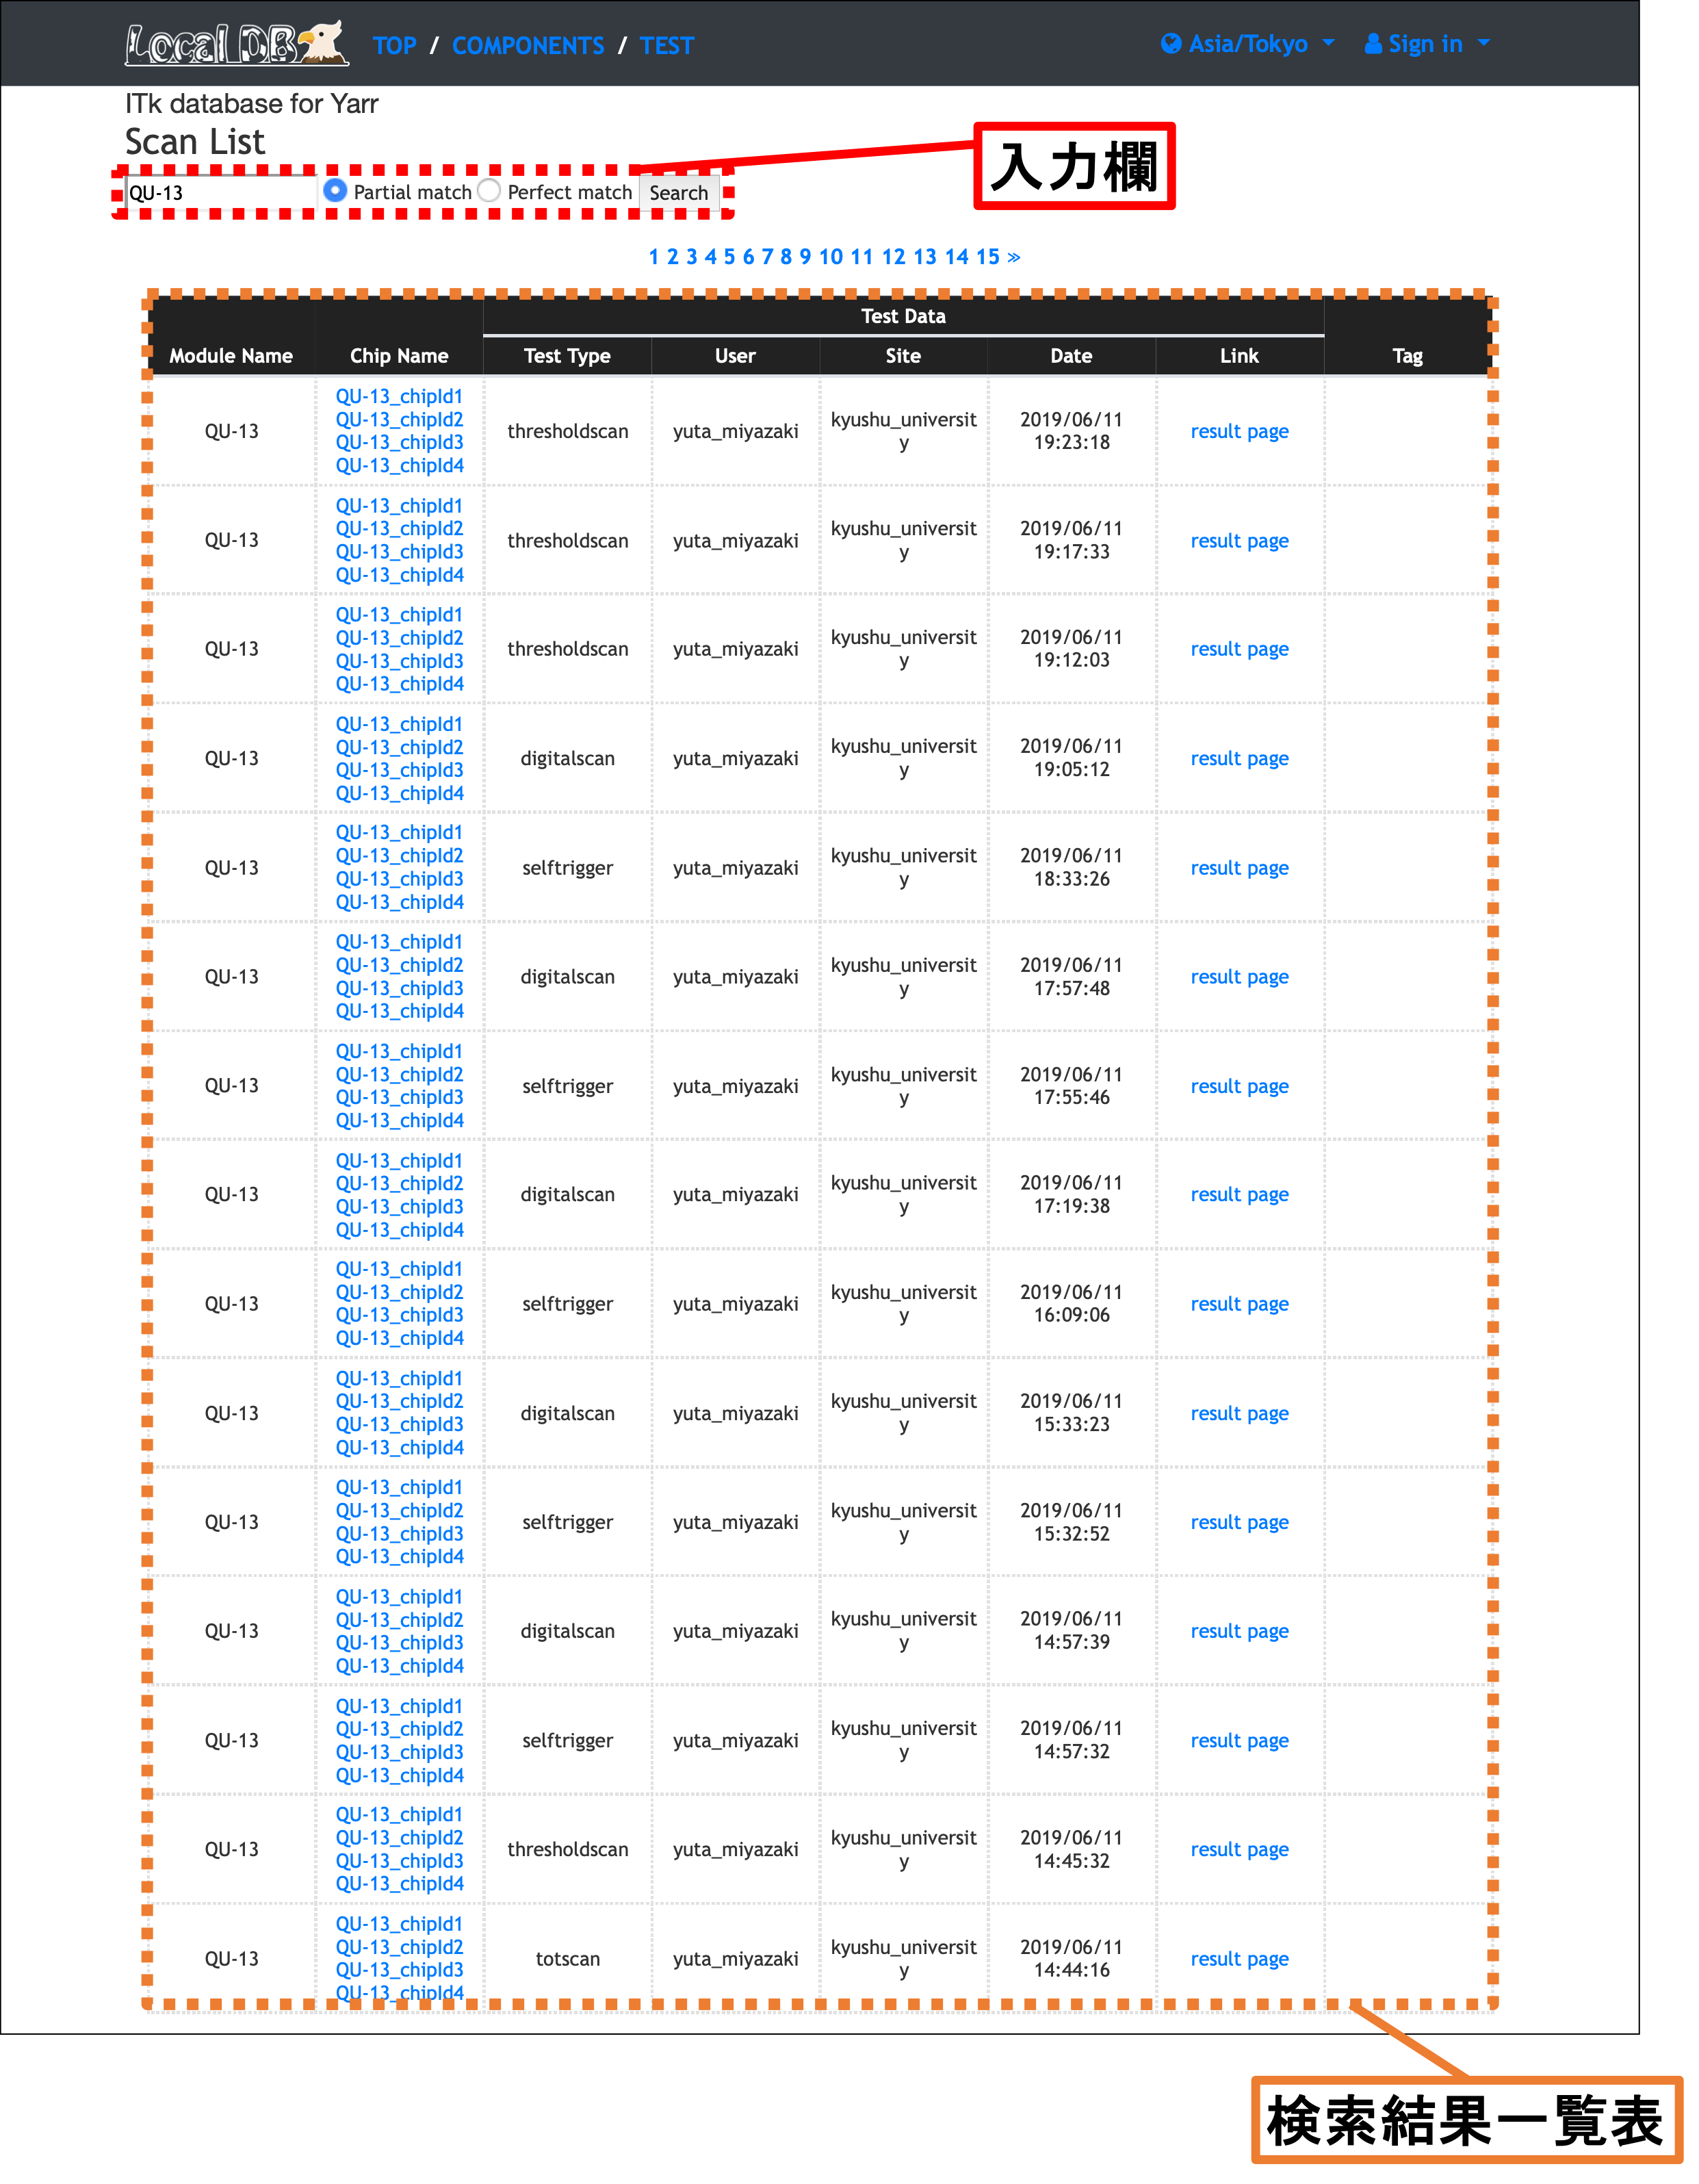
\includegraphics[width=9cm]{webapp_search_function}
\caption[ウェブアプリケーションにおける検索機能の様子]{ウェブアプリケーションにおける検索機能の様子。図は検索結果一覧表示のページである。図の上部に入力欄があり(赤破線)、ここにキーワードを入力し検索を実行する。図の例では"QU-13"と入力しており、検索結果にはモジュール名QU-13の試験結果が一覧表示されていることが分かる。}
\label{webapp_search_function}
\end{figure}

また生産に向けて、検索にかかる処理時間測定を行った。検索機能の詳しい実装方法と処理時間についての詳細は、6章で述べる。

%%%%%%%%%%%%%%%%%%%%%%%%%%%%%%%%%%%%%%%%%%%%%%%%%%%%%%%
%%%%%%%%%%%%%%%%%%%%%%%%%%%%%%%%%%%%%%%%%%%%%%%%%%%%%%%
\newpage
\subsection{中央データベースとの同期ツール}
生産時にはローカルデータベースと中央データベースにおいて、同期が必要となる。例えば、モジュール情報や組み立て工程、試験結果があげられる。
この同期を行うためのツールを開発した。主に開発した項目については以下の2つである。

\begin{itemize}
  \item モジュール及び構成するFEチップ情報のダウンロード機能
  \item 読み出し試験結果のアップロード機能
\end{itemize}

これらの機能のイメージを図\ref{interface_overview}に示す。
実装の詳細については8章で後述する。

\begin{figure}[bpt]\centering
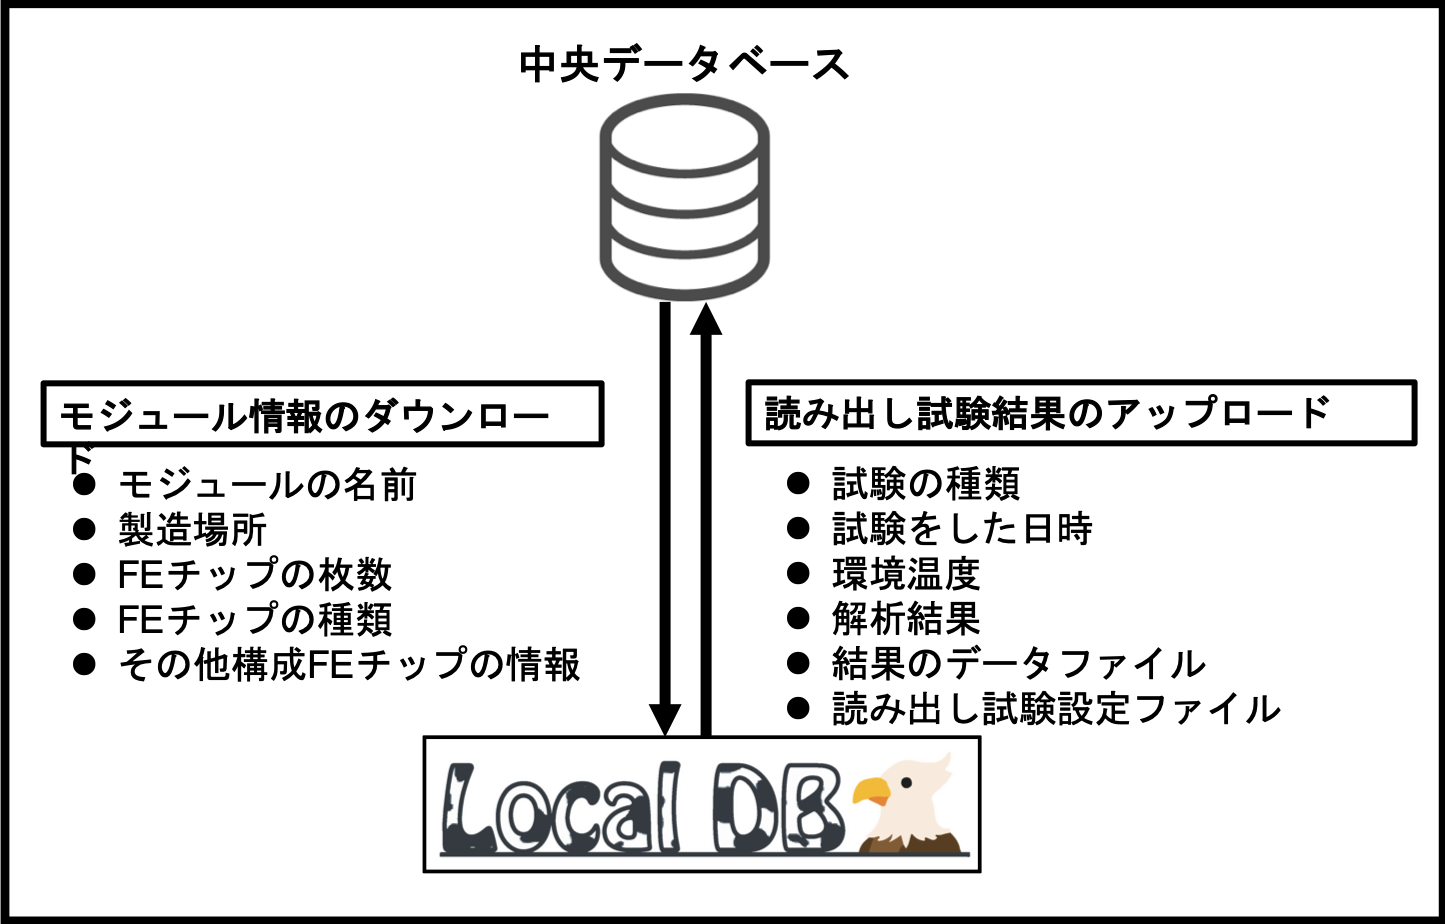
\includegraphics[width=12cm]{interface_overview}
\caption[同期機能の概要]{同期機能の概要。同期機能の中でも、本研究ではモジュール情報のダウンロードと読み出し試験結果のアップロード機能を実装した。図に示している情報を同期する機能となっている。}
\label{interface_overview}
\end{figure}

%%%%%%%%%%%%%%%%%%%%%%%%%%%%%%%%%%%%%%%%%%%%%%%%%%%%%%%
%%%%%%%%%%%%%%%%%%%%%%%%%%%%%%%%%%%%%%%%%%%%%%%%%%%%%%%
\newpage
\section{量産時の情報登録・同期の流れ}
量産時におけてデータベース操作は以下の流れで行うことを想定している。
\begin{enumerate}
  \item 中央データベースへモジュール登録及び登録情報のダウンロード
  \item 1で登録したモジュールに対して品質試験結果のローカルデータベースへのアップロード
  \item ステージ毎に品質試験結果の登録と中央データベースへアップロード
\end{enumerate}

流れのイメージを図\ref{dbsystem_flow}に示す。
品質試験結果のアップロードは各組み立て工程毎に行う。ローカルデータベースで品質試験結果を組み立て工程毎にまとめて扱い、各モジュールの現組み立て工程を正確に管理する目的がある。
\begin{figure}[bpt]\centering
  \begin{minipage}{0.5\hsize}
    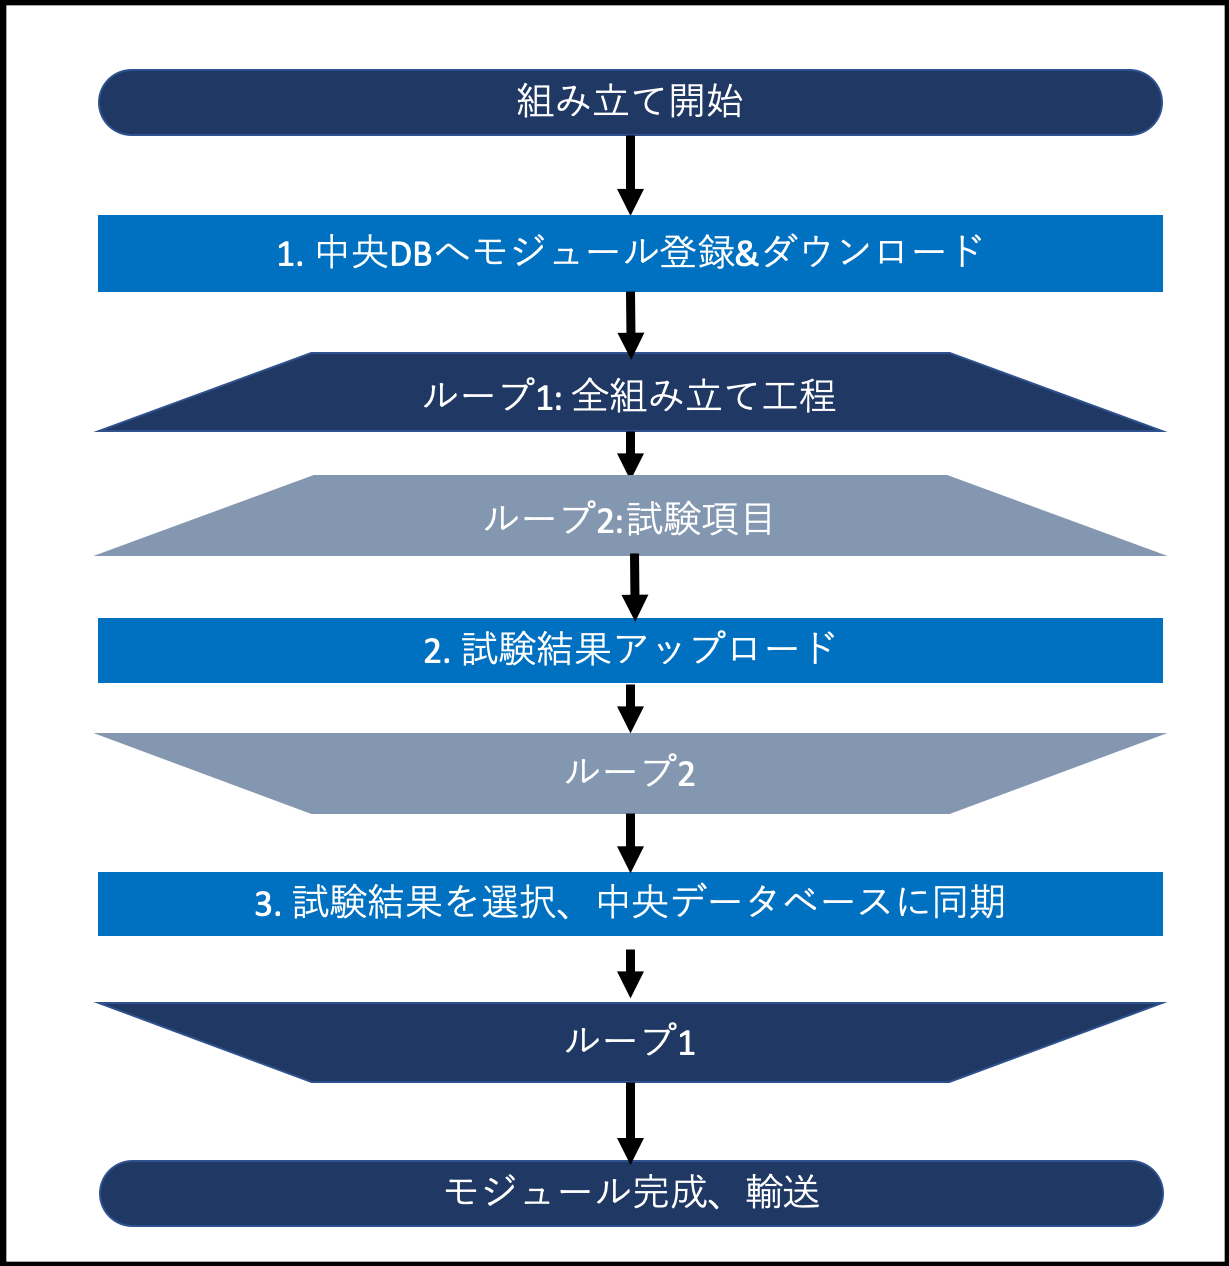
\includegraphics[width=7cm]{dbsystem_flowchart}
  \end{minipage}
  \begin{minipage}{0.4\hsize}
    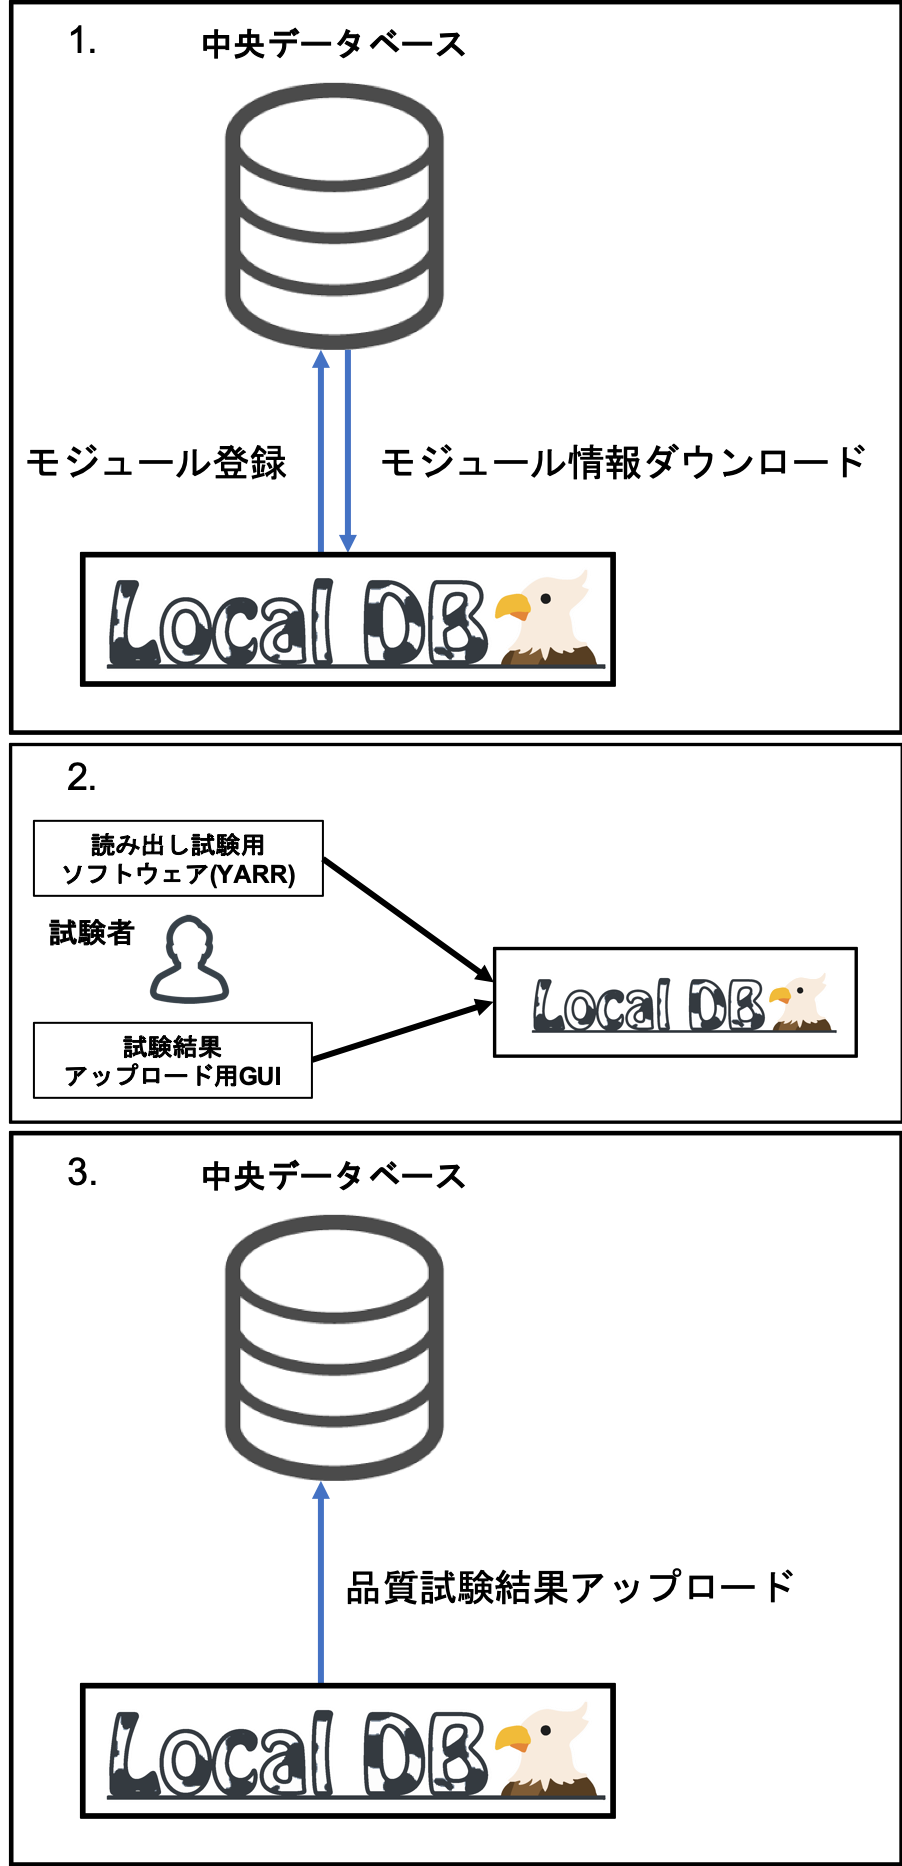
\includegraphics[width=5cm]{dbsystem_flow_image}
  \end{minipage}
\caption[各モジュールにおけるデータベースシステム操作の流れ]{各モジュールにおけるデータベースシステム操作の流れ。モジュール組み立てにおけるデータベース操作の初めに、中央データベースにモジュール登録及びローカルデータベースへモジュール情報のダウンロードを行う(処理1)。その後、ダウンロードしたモジュールに対して組み立て工程に応じた試験結果を生成、ローカルデータベースに保存する(処理2)。各組み立て工程の終わりに試験結果の選択を行い、中央データベースに試験結果を同期する(処理3)。}
\label{dbsystem_flow}
\end{figure}

全組み立て工程が終了すると、モジュールの情報及び品質試験結果が全て中央データベースへ同期されている状態となる。
データベース操作の流れの一部を学内実験室にて行った。詳細を5章で述べる。

\clearpage
\section{モジュール生産状況の解析}

上述したデータベースシステムを使って、モジュール生産状況の解析を行うことができる。
モジュールの組み立て工程は各生産場所のローカルデータベース上に記録され、組み立て工程ごとに中央データベースへ同期される。
そのため現在組み立てが行われている全てのモジュールの現在工程を中央データベース上で取得できることができ、この情報を用いて世界的な生産状況の解析を行うことができる。
現在は生産は行われていないが、想定している解析結果のイメージを図\ref{production_analysis}に示す。

\begin{figure}[bpt]\centering
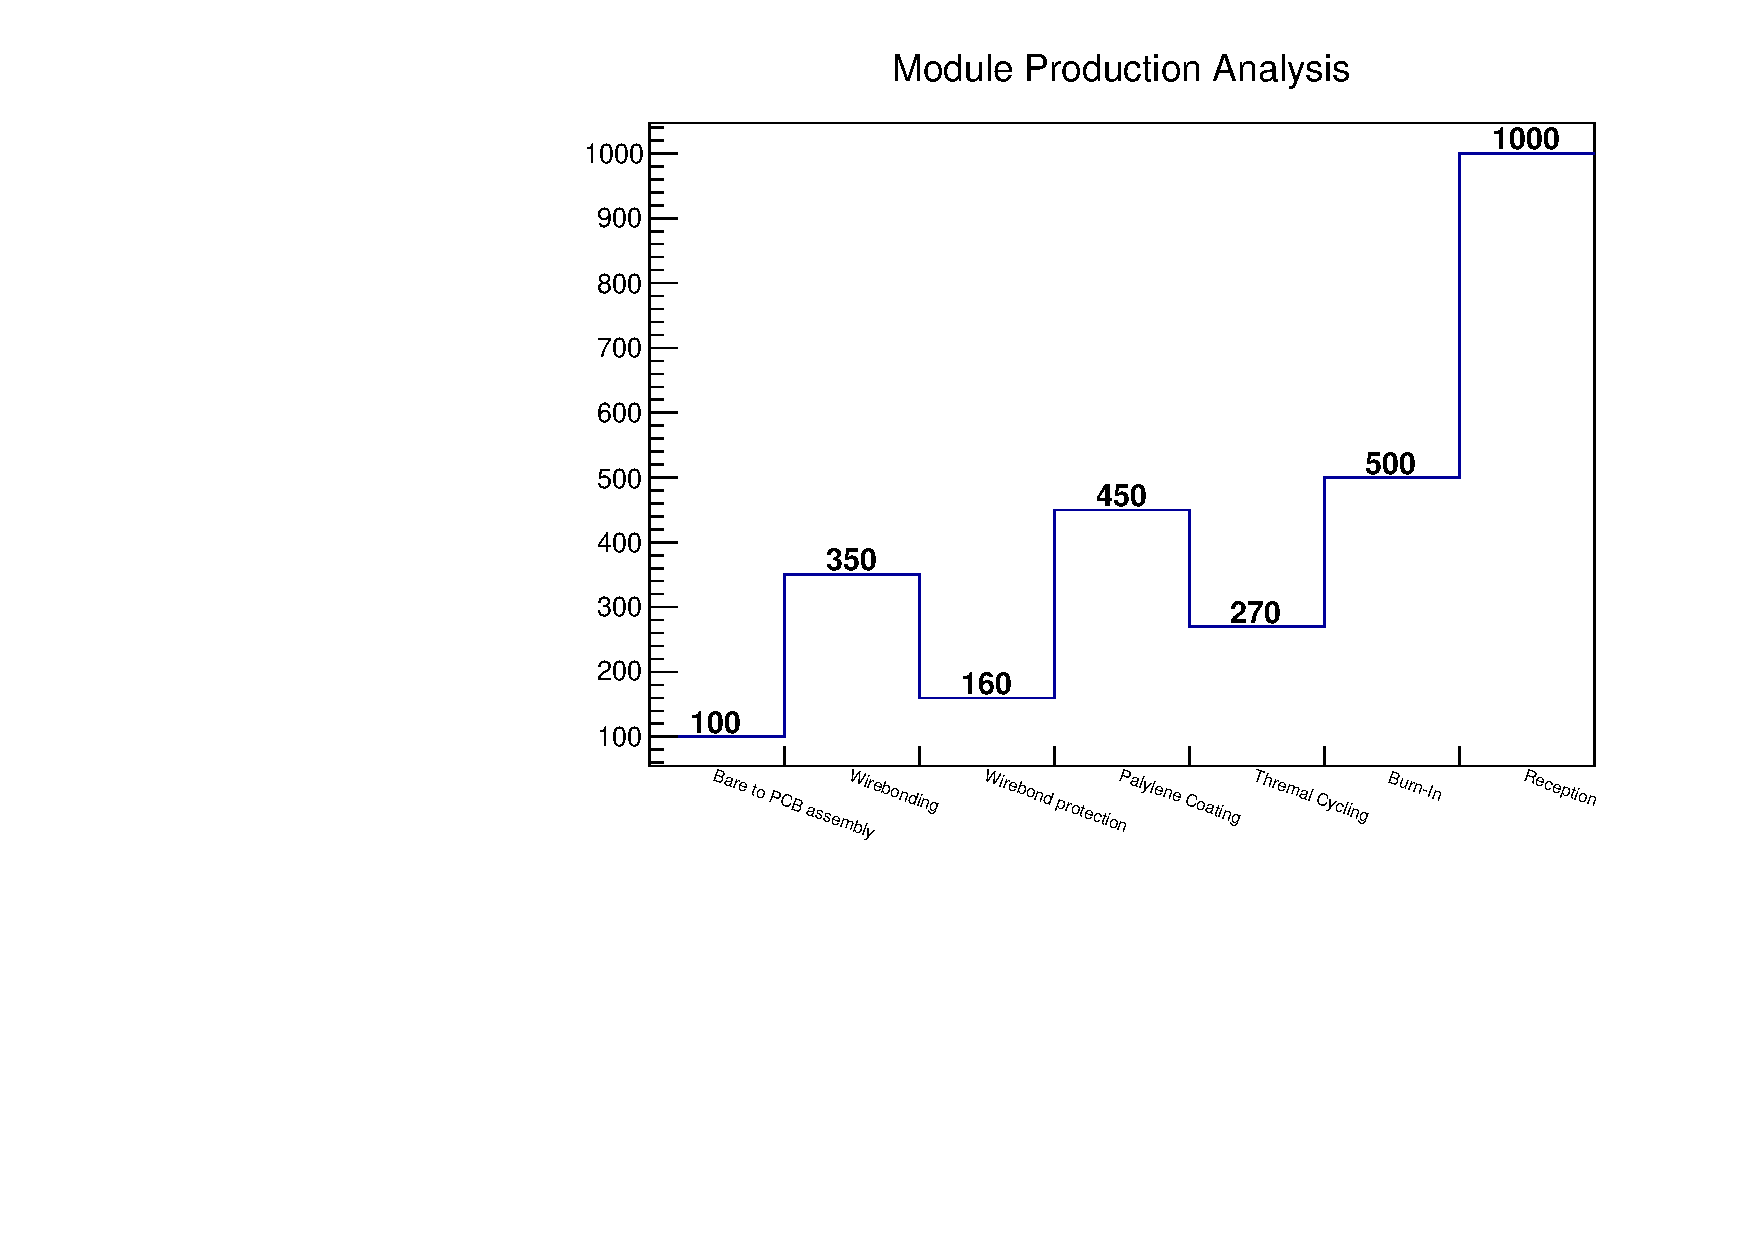
\includegraphics[width=8cm,angle=270]{production_analysis}
\caption[生産時のモジュール組み立て状況解析の例]{生産時のモジュール組み立て状況解析の例。ローカルデータベースにて組み立て工程は管理され、工程毎に中央データベースに同期されるため、生産時には全てのモジュールの現工程を中央データベースで取得できる。図の例ように各段階におけるモジュール数を見ることで生産状況の確認ができる。さらにある期間ごとに工程を取得することで生産レートなども計算することができ、今後の生産計画やモジュール選別の参考とすることができる。}
\label{production_analysis}
\end{figure}

生産数や生産レートのモニタリングを行うことで、今後の生産計画や問題解決に役立てることが可能である。

